\subsection{External Interface Requirements}

\subsubsection{User Interfaces}

\begin{figure} [H]
    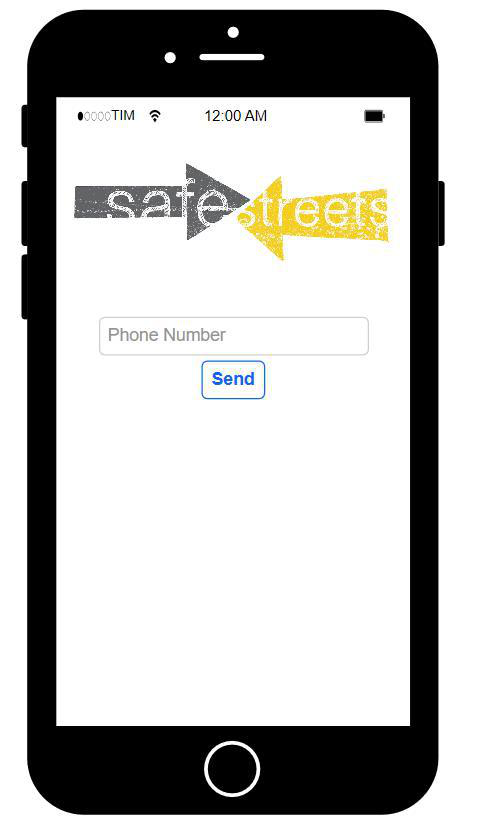
\includegraphics[scale=0.52]{Images/Templates/User/us_0.png}
    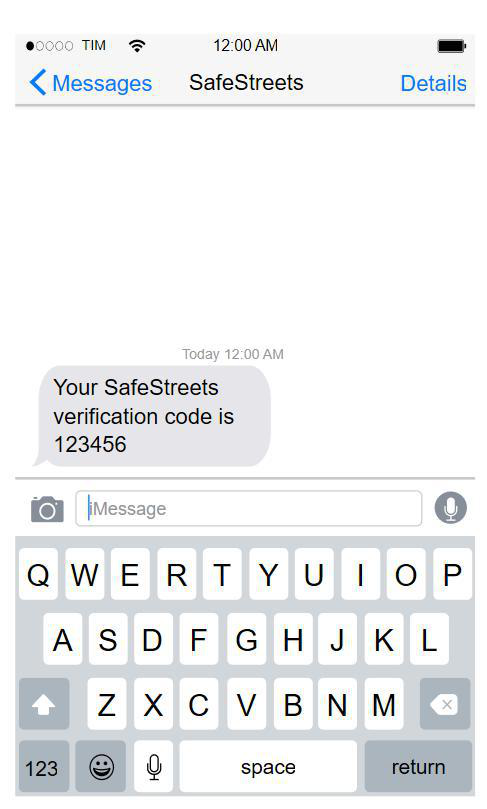
\includegraphics[scale=0.5]{Images/Templates/User/us_1.png}
    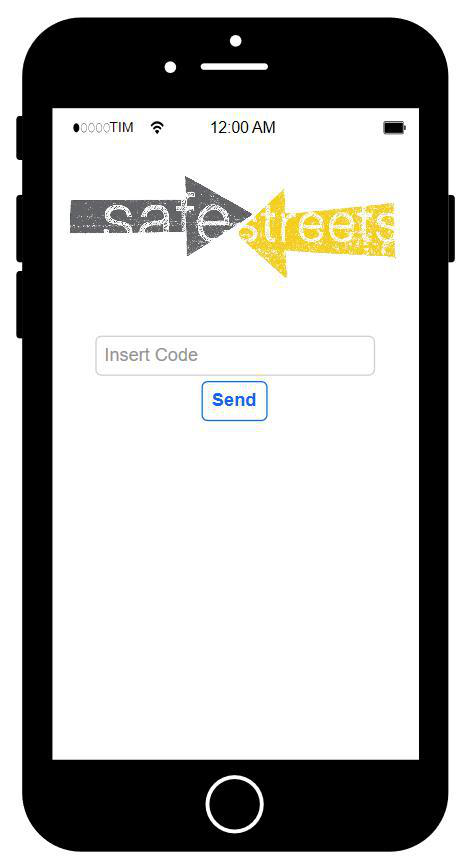
\includegraphics[scale=0.5]{Images/Templates/User/us_2.png}
    \caption{\label{fig:Mockup-1}Login}
\end{figure}

This is the first page the users are shown. To continue they 
have to input their cellphone number and to insert an OTP 
sent to them by the system.

\begin{figure} [H]
    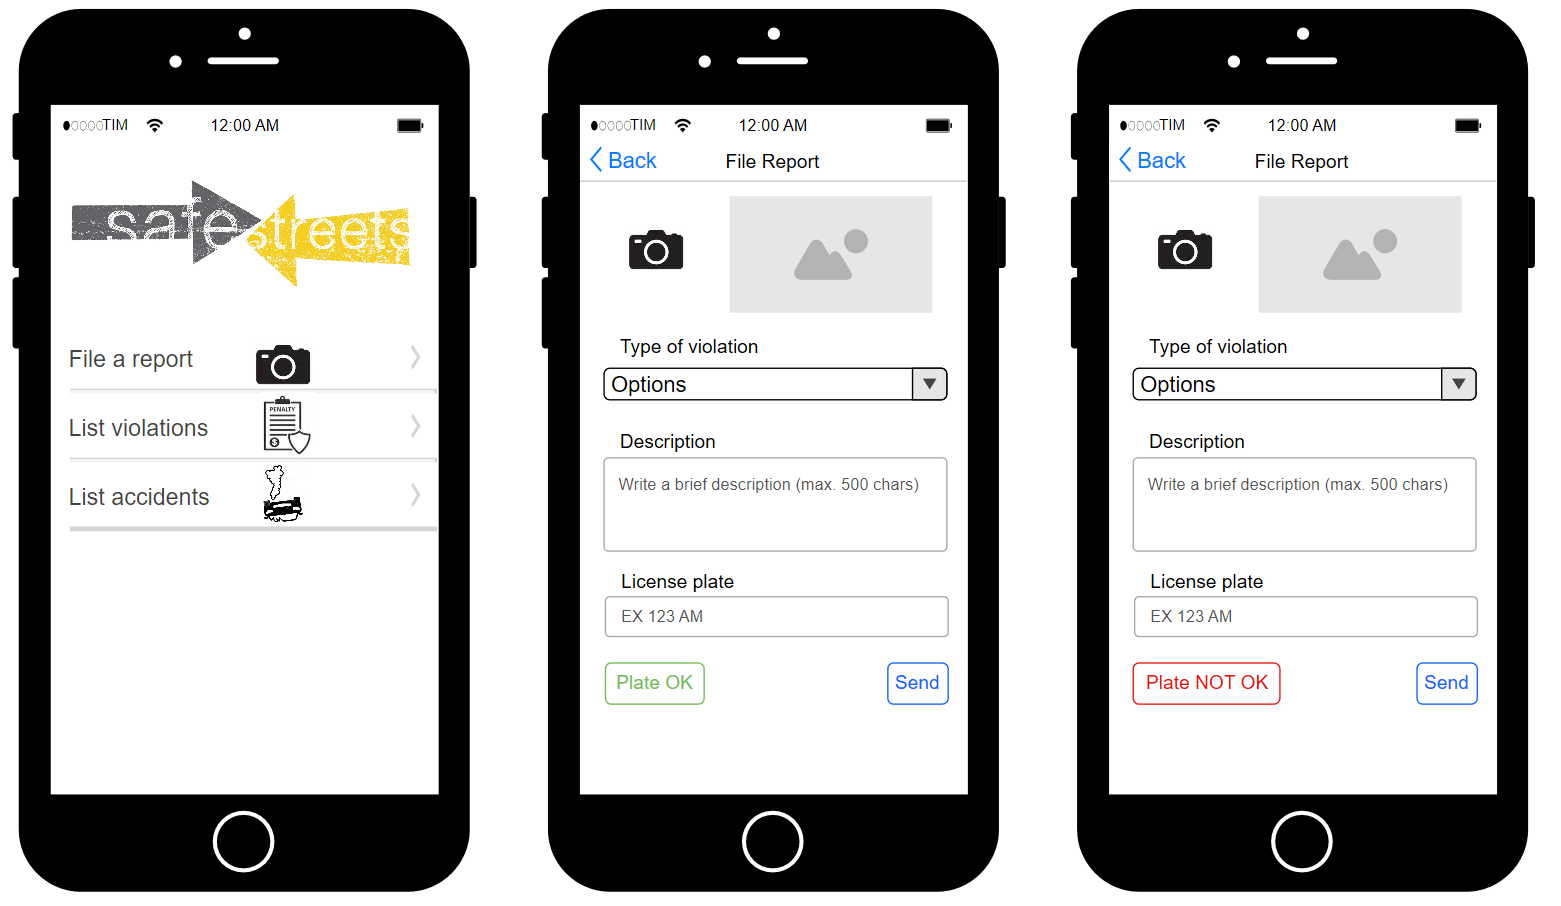
\includegraphics[scale=0.47]{Images/Templates/User/us_3.PNG}
    \caption{\label{fig:Mockup-2}Menu and File Report section}
    In this case it is shown how the report of violations is 
    handled. The users enters the correct area and fills all 
    the fields.
\end{figure}


\begin{figure} [H]
    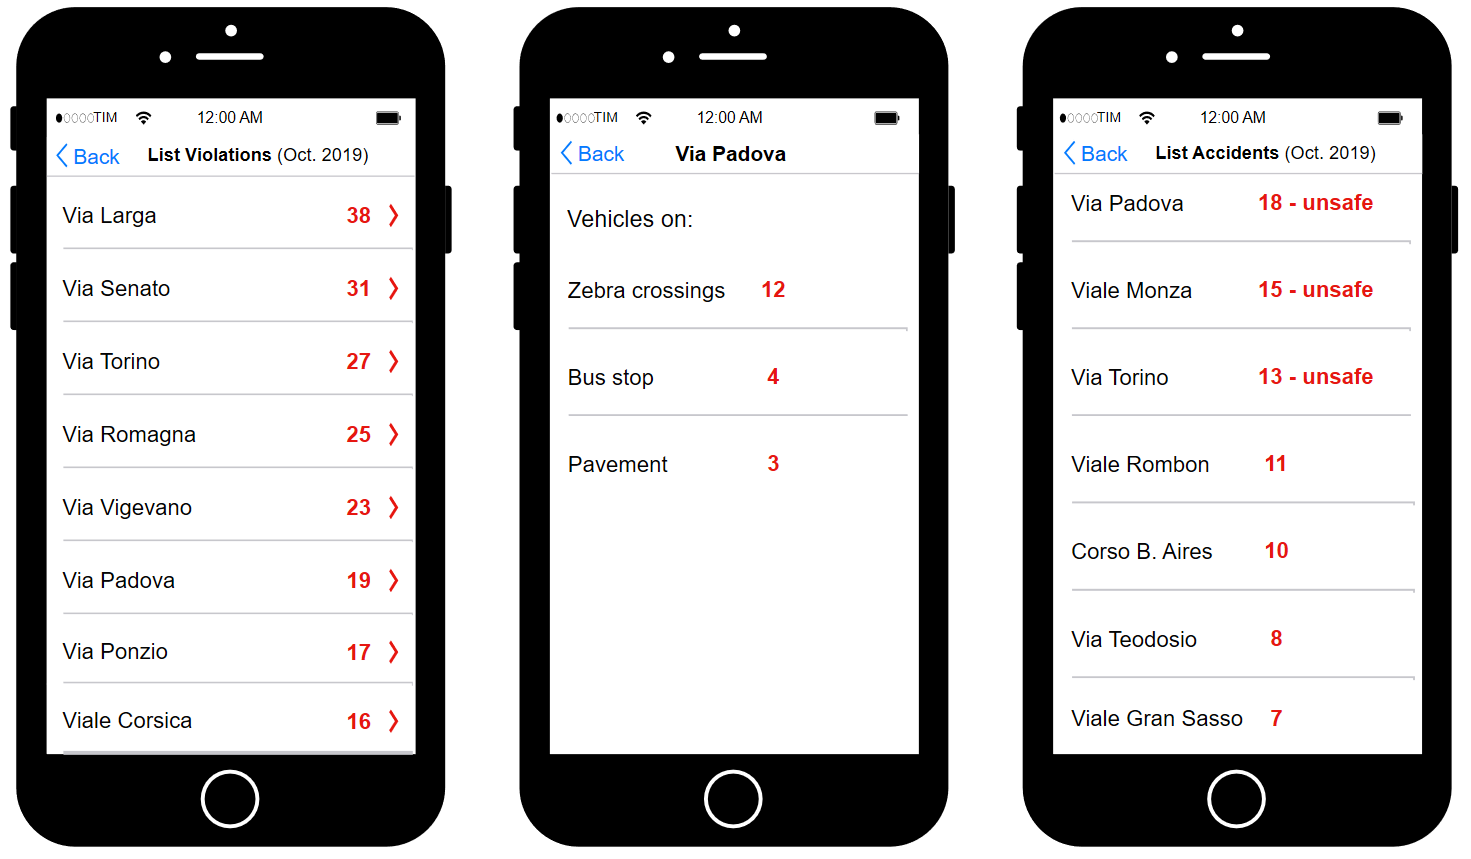
\includegraphics[scale=0.5]{Images/Templates/User/us_4.PNG}
    \caption{\label{fig:Mockup-3}List Violations and List 
    Accidents sections}
    Upon entering on the apposite areas, the users are shown 
    a list of streets with information about violations. If 
    a precise one is selected, the types are linked to their 
    quantities.
\end{figure}


\subsubsection{Authority Interfaces}
\begin{figure} [H]
    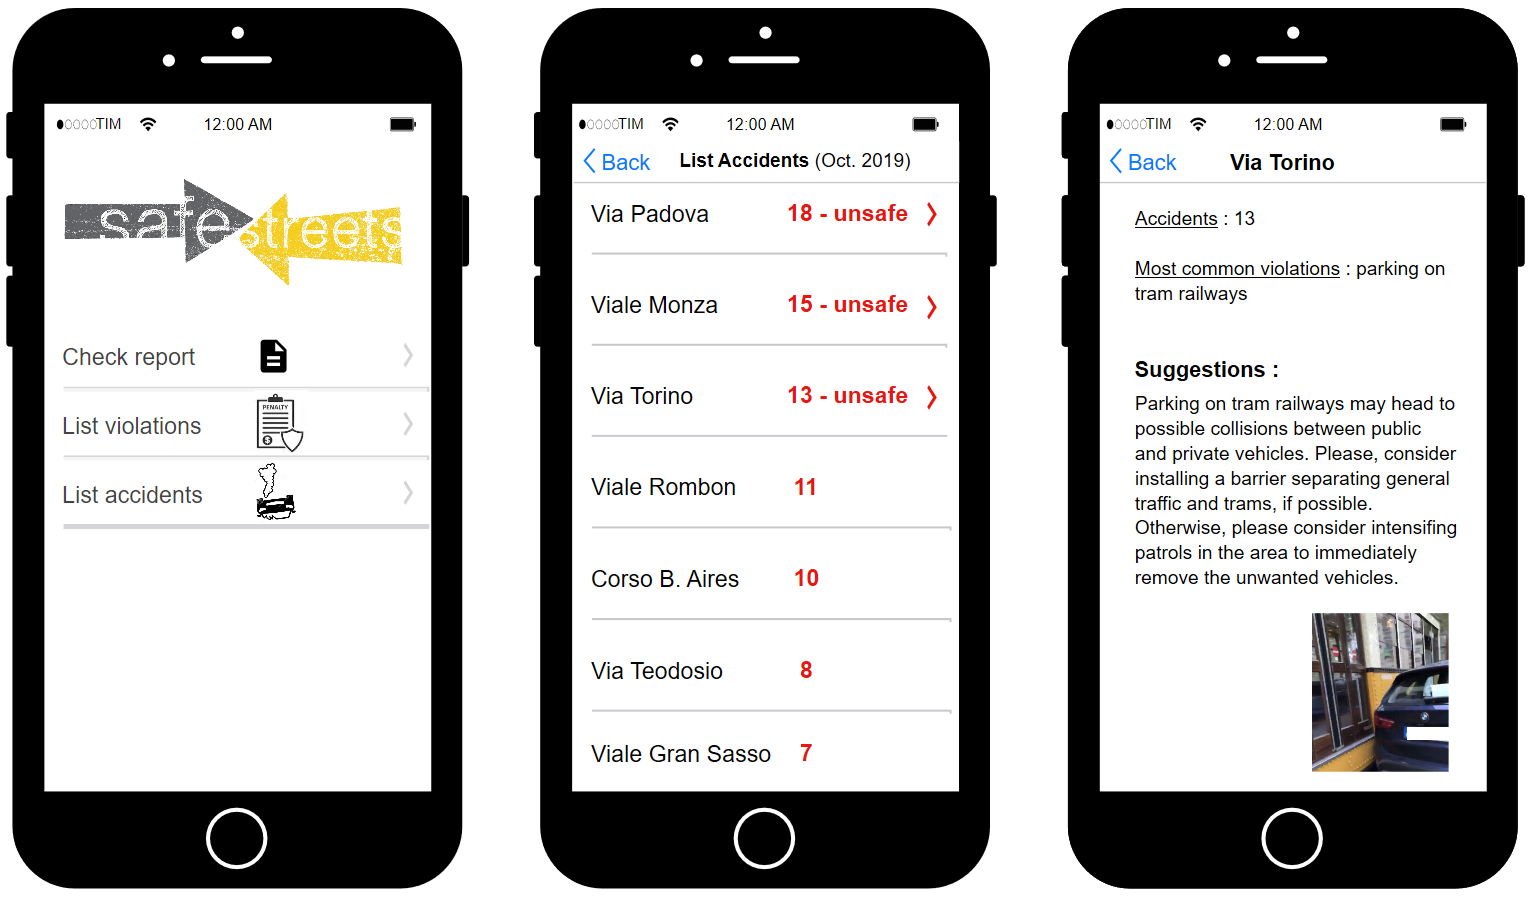
\includegraphics[scale=0.48]{Images/Templates/Authority/auth_0.PNG}
    \caption{\label{fig:Mockup-4}Menu and List Accidents section}
\end{figure}

Authorities can select unsafe streets from the section regarding 
accidents. If said street is listed as \textit{unsafe}, the type 
of most common violations is shown. A suggestion is made accordingly, 
as it can be argued that if drivers tend to reiterate a specific mistake, 
it is possible that this is the cause of the accidents.

\begin{figure} [H]
    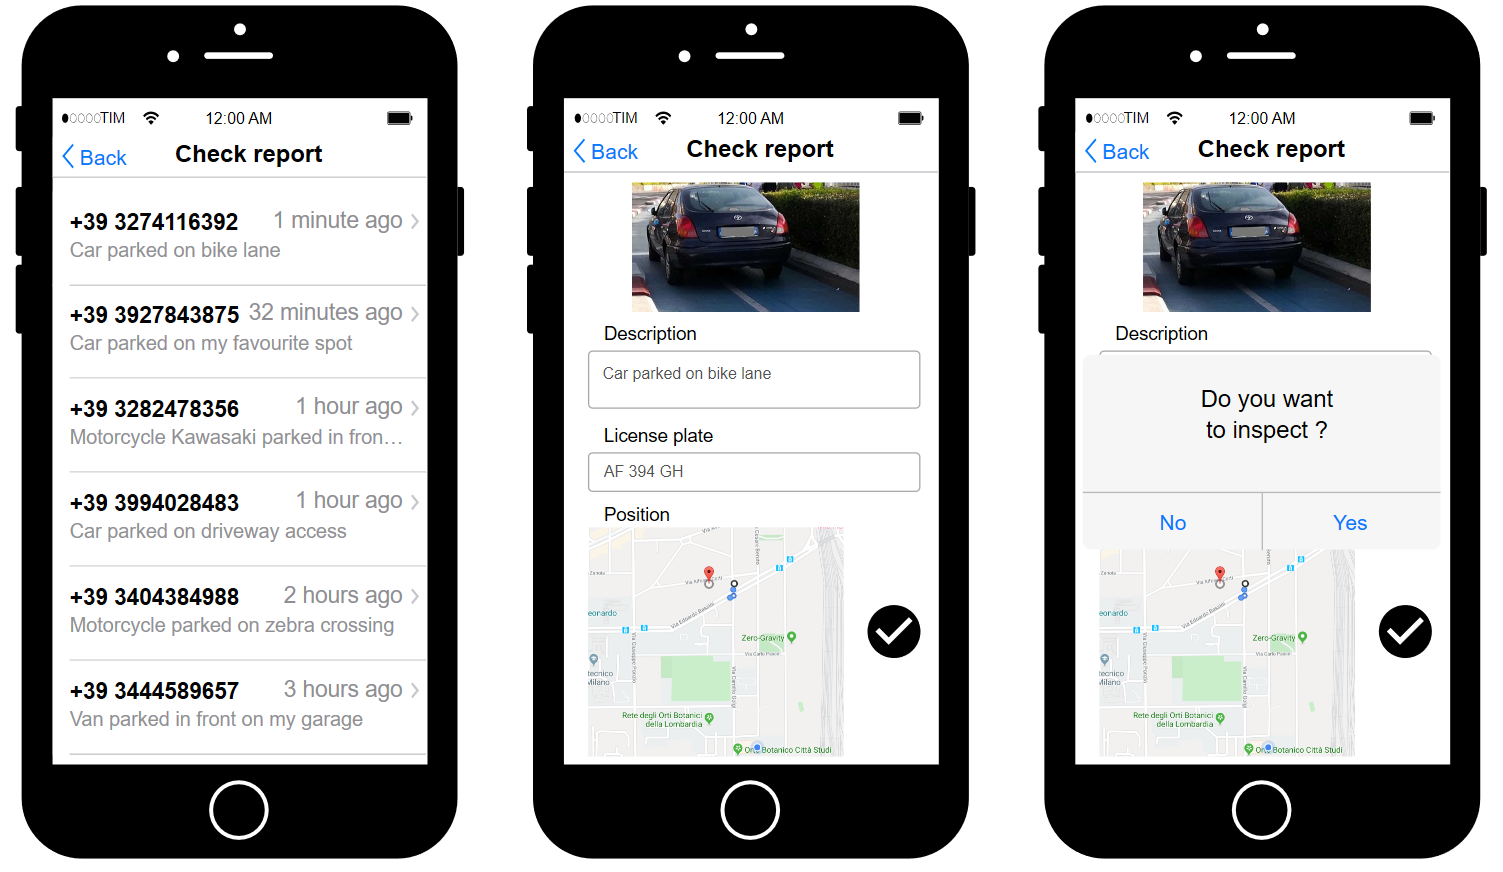
\includegraphics[scale=0.49]{Images/Templates/Authority/auth_1.PNG}
    \caption{\label{fig:Mockup-5}Check Report section}
\end{figure}

Authorities can discard specific violations or take them in charge. 
If the latter happens, they are guided to the site of the violation 
exploiting GM' API.

\begin{figure} [H]
    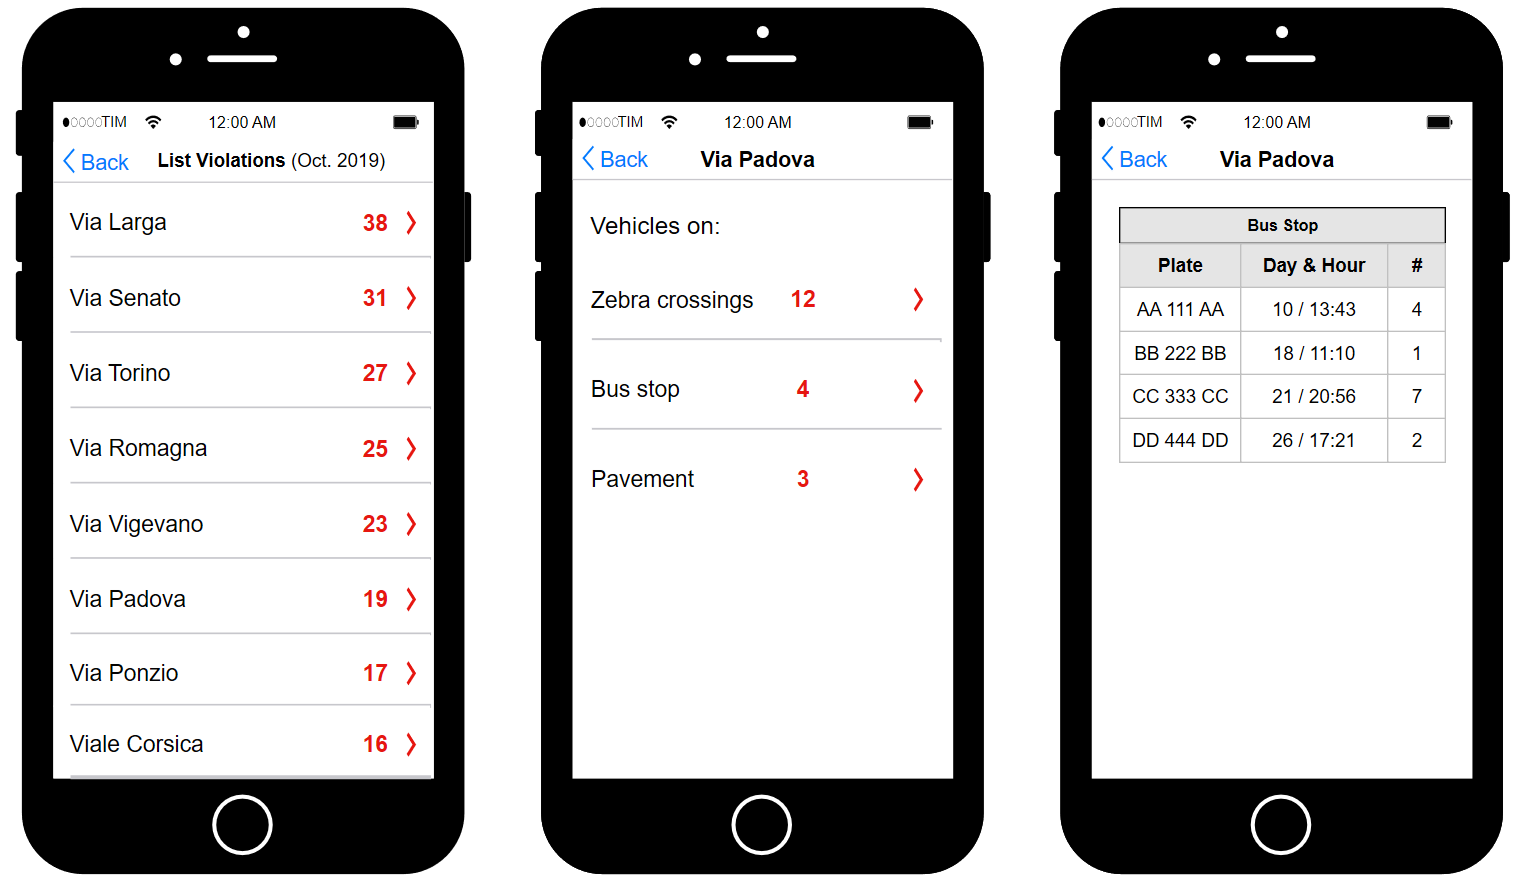
\includegraphics[scale=0.48]{Images/Templates/Authority/auth_2.PNG}
    \caption{\label{fig:Mockup-6}List Violations section}
\end{figure}

Authorities can see the list of the offenders, street by street, 
for any kind of violation.

\begin{figure} [H]
    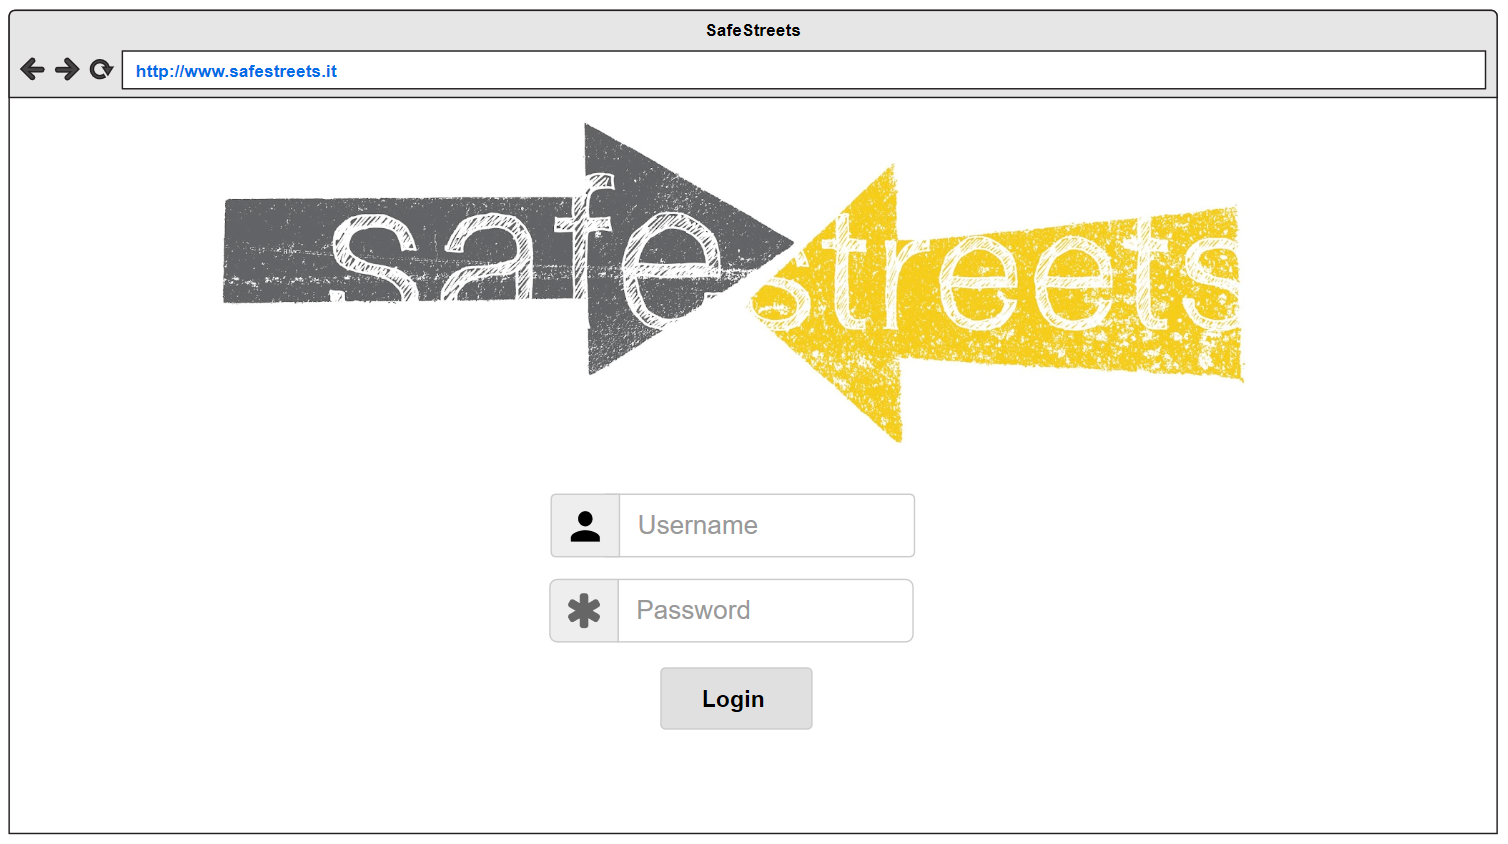
\includegraphics[scale=0.5]{Images/Templates/Authority/auth_3.PNG}
    \caption{\label{fig:Mockup-7}Web Login interface}
\end{figure}

Safestreets is provided with a web interface for those authorities 
who are assigned to administrative section.

\begin{figure} [H]
    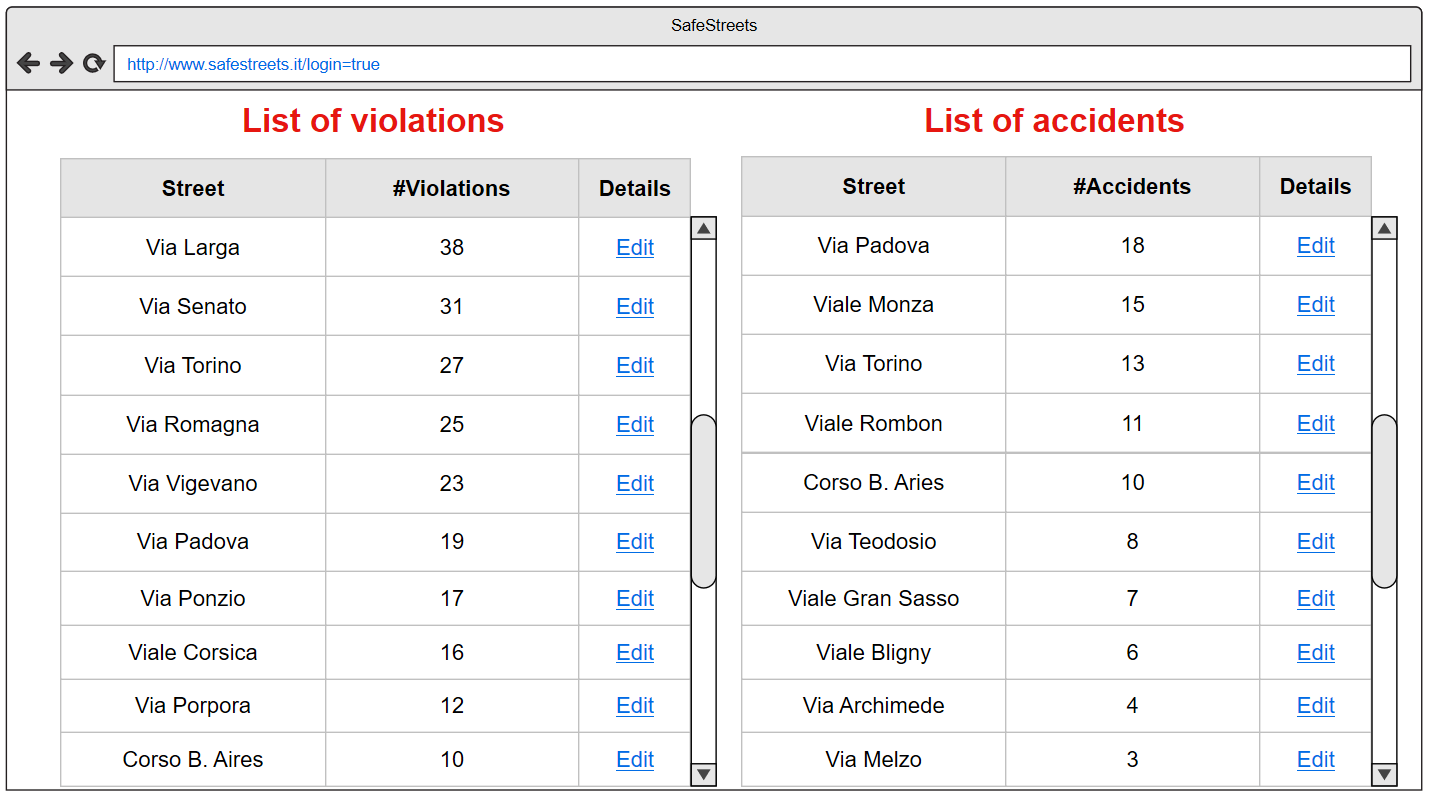
\includegraphics[scale=0.5255]{Images/Templates/Authority/auth_4.PNG}
    \caption{\label{fig:Mockup-8}Web interface}
\end{figure}

This version is used merely for data analysis and inspection.

\subsubsection{Hardware Interfaces}

The application is available to those who have a smartphone with internet 
connection (to communicate with SafeStreet), a camera (to take photos of 
the violations) and a GPS tracker (to provide the position).
The web application for authorities can be accessed by any computer with 
a web browser.

\subsubsection{Software Interfaces}

\begin{itemize}
    \item Browser
    \item Web Server Application
    \item Operating System: iOS, Android
    \item DBMS
\end{itemize} 

\subsubsection{Communication Interfaces}

This application requires an Internet connection for the purpose of 
transmitting the report information, HTTPS protocol is used to transfer 
the data securely between the user and the DBMS.

\subsection{Functional Requirements}
\begin{outline}

    \1 \textbf{G1} The application has to store all the information about 
    violations sent to it, until a ticket is either dropped or accepted 
    by an authority
    \2 \textbf{D5}: There is no failure in communication
    \2 \textbf{D7}: Data storage is reliable
    \2 \textbf{R1}: Users must login to SafeStreets

%____________________________________________________________________________

    \1 \textbf{G2} The system must accepts violations issued from every 
    part of the covered area
    \2 \textbf{D1}: The smartphone of the user can provide accurate 
    location
    \2 \textbf{D3}: Internet connection is reliable
    \2 \textbf{D4}: There is no failure in communication
    \2 \textbf{R2}: Users must be connected to the internet with their 
    GPS enabled to use the service
    \2 \textbf{R3}: Users must fill the log to send a report

%____________________________________________________________________________
    
    \1 \textbf{G3} The system must allow authorities to access 
    violations in every part of the covered area
    \2 \textbf{D3}: Internet connection is reliable
    \2 \textbf{D5}: There is no failure in communication
    \2 \textbf{D6}: GM is always on and ready to communicate
    \2 \textbf{D7}: Data storage is reliable
    \2 \textbf{R4}: Authorities must be connected to the internet with 
    their GPS enabled to use the service
    \2 \textbf{R5}: Authorities must login to use Safestreets
    \2 \textbf{R6}: Authorities can close open reports 

%____________________________________________________________________________

    \1 \textbf{G4} The application allows users and authorities 
    to mine information on the system
    \2 \textbf{D3}: Internet connection is reliable
    \2 \textbf{D5}: There is no failure in communication
    \2 \textbf{D7}: Data storage is reliable
    \2 \textbf{R6}: Users are able to retrieve info about violations 
    for every street
    \2 \textbf{R7}: Users are able to retrieve info about violations 
    for every street
    \2 \textbf{R8}: Authorities are able to retrieve info about violations 
    for every street
    \2 \textbf{R9}: Authorities are able to retrieve info about violations 
    for every street

%____________________________________________________________________________

    \1 \textbf{G5} The application identifies unsafe areas crossing 
    its informations with those offered by the municipality
    \2 \textbf{D7}: Data storage is reliable
    \2 \textbf{D8}: Data offered by municipality is correct
    \2 \textbf{D9}: Data offered by municipality is up-to-date
    \2 \textbf{R10}: The system can store data permanently 

%____________________________________________________________________________

    \1 \textbf{G6} The application suggests possible solution to 
    problems perceived after the crossing of information
    \2 \textbf{D2}: The data provided by the user is correct
    \2 \textbf{D8}: Data offered by municipality is correct
    \2 \textbf{D9}: Data offered by municipality is up-to-date
    \2 \textbf{R10}: The system can store data permanently 


\end{outline}

\subsubsection{Scenarios}

\subsubsection*{Scenario A}

Alberto, while on on his way to the workplace, notices a car parked 
on the zebra crossing so he decides to use Safestreets to report it. 
He inserts his number on the homepage of the app, then he fills the 
following field with the OTP sent to him by SMS. He takes a photo of 
the car while he is fare from it,but the "PLATE NOT OK" signal appears 
on the bottom.He tries again, this time getting nearer and carefully 
framing the license plate. The number appears correctly on the page 
(AA 000 AA), so he just chooses the type of the violation ("Parking on 
zebra crossings") and writes a brief description "Car parked in a critical 
spot right in front of a school". The GPS on the map points to "Via Goito 4", 
he clicks on "Send" and the violation is sent to the server, waiting for someone 
to take it in charge.
As he wants to know if that type of violation is common in that area, he selects 
"List Violations" and then he goes on the section dedicated to Via Goito. He 
reads that the most common violation there is indeed "Parking on zebra crossing" 
followed by "Double parking" so he realizes that he should look out for these 
errors while waling on the street.

\subsubsection*{Scenario B}

Bernardo has just taken the driving license and wants to use his car to reach 
a friend living on the other side of the city. As he has not much experience 
yet, he decides to calculate a path to said part before getting behind the 
wheel. He opens SafeStreets and, after the login procedure, he checks the 
list of accidents of the city. He sees that the streets on which his friend 
lives is unsafe and it is subject to a great deal of parking violations. 
He realizes that he wants to avoid that street as he wants to sharpen his skills 
before and that parking there is unfavourable, so he calculates a new path and 
finds a more suitable street to park in.

\subsubsection*{Scenario C}

Chiara is a policewoman patrolling the streets near the Duomo, she decides to 
open SafeStreets to find any violation to sanction. She logs in using her 
credentials and she goes on the section "Check Reports". She reads a report 
of a moped double parked on Via Torino 23 and she goes to check (using the map 
on the app). She wants to check if that vehicle has already committed another 
violation, so she goes on the "List Violation" section and highlights Via Torino. 
She reads that the proprietary of the vehicle has already double parked on the same 
street. She calls the service for the removal of the moped and she takes in charge 
the report; it is kept on the DB.

\subsubsection*{Scenario D}

Dario works at the Comando Pulizia Municipale and he is currently revisioning the safety 
of the streets in the city. To speed the process up he logs on to the webpage of 
SafeStreets and checks the list of accidents. He finds that a few streets are marked as 
unsafe, as they have registred a number of accidents over \tres . He selects said parts 
and reads the suggestions listed. Deeming them reasonable, he writes a reports to his 
boss suggesting these changes and waits for them to be implemented.

\subsubsection{Use Case Diagrams}

\begin{figure}[H]
    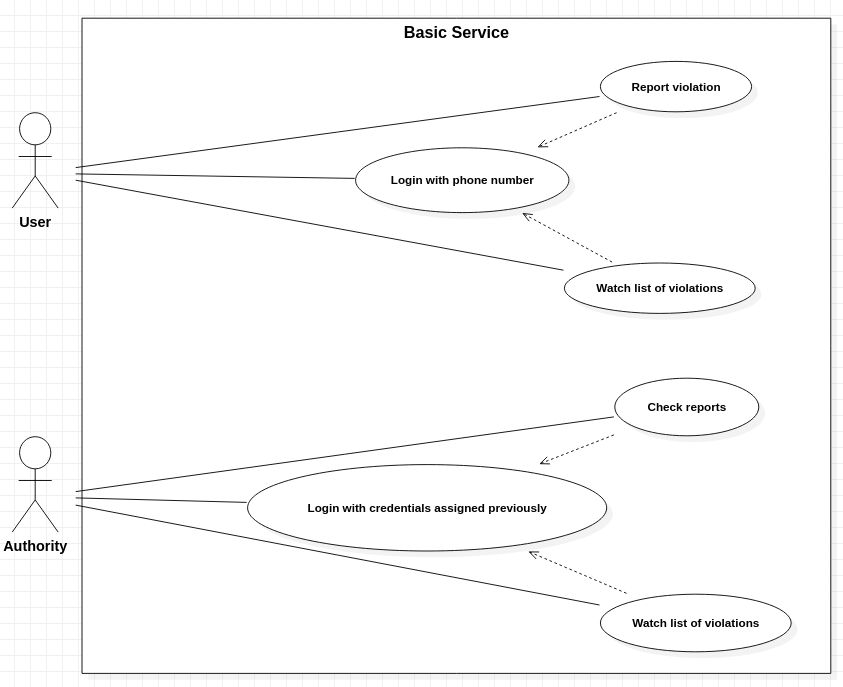
\includegraphics[scale=0.41]{Images/Diagrams/UseCase1.png}
    \caption{\label{fig:UseCase1}SafeStreets basic service use case diagram}
\end{figure}

\begin{figure}[H]
    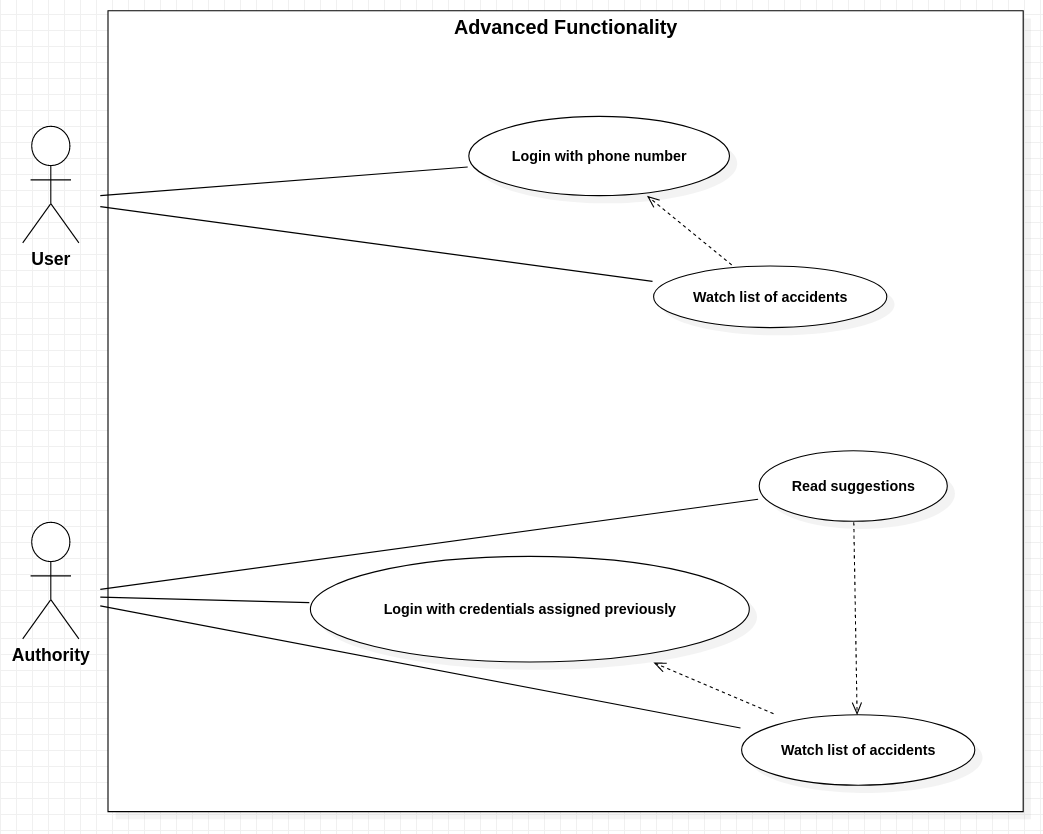
\includegraphics[scale=0.34]{Images/Diagrams/UseCase2.png}
    \caption{\label{fig:UseCase2}SafeStreets advanced functionality use case diagram}
\end{figure}

\subsubsection{Use Case} 

\vspace{1cm}

\begin{flushleft}
\begin{tabular}{|c|l|}
\hline
    \textbf{Name} & Login with phone number\\ \hline
    \textbf{Actor} & User\\ \hline
    \textbf{Entry conditions} & The user has installed the application on their device\\ \hline
    \textbf{Events flow} 
    & 1. The user inserts their phone number\\ 
    & 2. The user taps on 'send'\\ 
    & 3. The user receives an SMS with an OTP\\ 
    & 4.The user inputs the OTP\\ 
    & 5. The user taps on 'send'\\ \hline
    \textbf{Exit conditions} &  The user logins and is prompted with the interface of 
    the App\\ \hline
    \textbf{Exceptions} 
    & 1. The user uses an invalid phone number\\
    & 2. The user inputs an invalid OTP\\ 
\hline 
\end{tabular}
\end{flushleft} 

\vspace{1.5cm}

\begin{flushleft}
\begin{tabular}{|c|l|}
\hline
    \textbf{Name} & Login with credentials assigned previously\\ \hline
    \textbf{Actor} & Authority\\ \hline
    \textbf{Entry conditions} & The authority was provided with credentials\\ \hline
    \textbf{Events flow} 
    & 1. The authority inputs their username\\
    & 2. The authority inputs their password\\
    & 3. The authority taps on 'login'\\ \hline
    \textbf{Exit conditions} & The authority logins and is prompted with the interface of the App\\ \hline
    \textbf{Exceptions} 
    & 1. The authority inputs a wrong username\\
    & 2.The authority inputs a wrong password\\
\hline 
\end{tabular} 
\end{flushleft}

\vspace{1.5cm}

\begin{flushleft}
\begin{tabular}{|c|l|}
\hline
    \textbf{Name} & Report violation\\ \hline
    \textbf{Actor} & User\\ \hline
    \textbf{Entry conditions} &  The user is logged in\\ \hline
    \textbf{Events flow} & 
    1. The user selects 'file a report' on the menu\\
    & 2. The user taps on the camera icon\\
    & 3. The user takes a photo of the violation\\
    & 4. The user selects the type of violation\\
    & 5. The user writes a brief description\\
    & 6. The user corrects the license plate(if incorrect)\\
    & 7. The user taps on 'send'\\ \hline
    \textbf{Exit conditions} 
    & The user is notified the success of the operation and is brought back\\ 
    & to the main menu\\ \hline
    \textbf{Exceptions} 
    & 1. The user doesn't fill all the fields\\
    & 2. The user has already filed a report and it has not been closed yet\\
\hline 
\end{tabular}
\end{flushleft}

\newpage

\begin{flushleft}
\begin{tabular}{|c|l|}
\hline
    \textbf{Name} & Check reports\\ \hline
    \textbf{Actor} & Authority\\ \hline
    \textbf{Entry conditions} &  The authority is logged in\\ \hline
    \textbf{Events flow} 
    & 1. The authority selects 'check report' on the menu\\
    & 2. The authority selects a report\\
    & 3. The authority accepts or discards the report\\ \hline
    \textbf{Exit conditions} 
    & The authority stays on the page and can choose later to close or\\
    & eliminate the report\\ \hline
    \textbf{Exceptions} & \\
\hline 
\end{tabular} 
\end{flushleft}

\begin{flushleft}
\begin{tabular}{|c|l|}
\hline
    \textbf{Name} & Watch list of violations\\ \hline
    \textbf{Actor} & User\\ \hline
    \textbf{Entry conditions} &  The user is logged in\\ \hline
    \textbf{Events flow} 
    & 1. The user selects 'list violations' on the menu\\
    & 2. The user taps on a specific street\\ \hline
    \textbf{Exit conditions} &  The user can see the types of violation with the respective values\\ \hline
    \textbf{Exceptions} & No violation occured the previous month\\
\hline 
\end{tabular}
\end{flushleft}

\begin{flushleft}
\begin{tabular}{|c|l|}
\hline
    \textbf{Name} & Watch list of violations\\ \hline
    \textbf{Actor} & Authority\\ \hline
    \textbf{Entry conditions} &  The authority is logged in\\ \hline
    \textbf{Events flow} 
    & 1. The authority selects 'list violations' on the menu\\
    & 2. The authority taps on a specific street\\
    & 3. The authority taps on a specific type of violation\\ \hline
    \textbf{Exit conditions} &  The authority can see the list of the repeated offenders\\ \hline
    \textbf{Exceptions} & No violation occured the previous month\\
\hline 
\end{tabular} 
\end{flushleft}

\begin{flushleft}
\begin{tabular}{|c|l|}
\hline
    \textbf{Name} & Watch list of accidents\\ \hline
    \textbf{Actor} & User\\ \hline
    \textbf{Entry conditions} & The user is logged in\\ \hline
    \textbf{Events flow} & The user selects 'list accidents' on the menu\\ \hline
    \textbf{Exit conditions} 
    & The user can see the list of the streets with the respective number of\\
    & accidents, marked the most unsafe\\ \hline
    \textbf{Exceptions} & No accident occured the previous month\\
\hline 
\end{tabular}
\end{flushleft}

\begin{flushleft}
\begin{tabular}{|c|l|}
\hline
    \textbf{Name} & Watch list of accidents\\ \hline
    \textbf{Actor} & Authority\\ \hline
    \textbf{Entry conditions} & The authority is logged in\\ \hline
    \textbf{Events flow} 
    & 1. The authority selects 'list accidents' on the menu\\
    & 2. The authority selects one of the unsafe streets listed\\ \hline
    \textbf{Exit conditions} 
    & The authority can see the number of accidents, the most common\\
    & type of violation and suggestions for the street\\ \hline
    \textbf{Exceptions} 
    & 1. No accident occured the previous month\\
    & 2. No street registered at least 12 accidents\\
\hline 
\end{tabular}
\end{flushleft}

\subsubsection{Sequence Diagram}
\begin{figure} [H]
    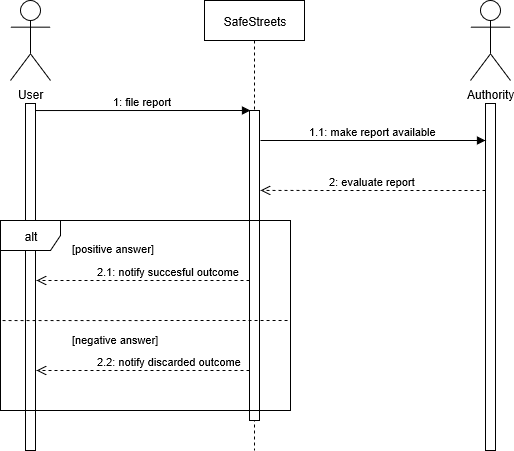
\includegraphics[scale=0.5]{Images/Diagrams/Sequence1.png}
    \caption{\label{fig:Sequence1}Lifetime of a report}
\end{figure}

\begin{figure} [H]
    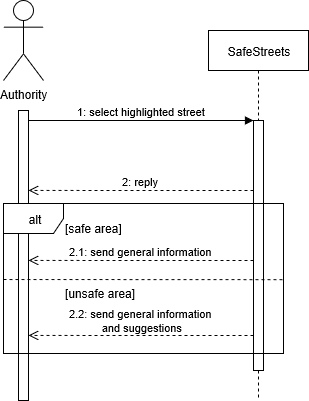
\includegraphics[scale=0.5]{Images/Diagrams/Sequence2.png}
    \caption{\label{fig:Sequence2}Examination of accidents}
\end{figure}

\subsection{Performance Requirements}

The system must be able to handle large quantities of data. 
On the other hand the importance of speed is limited as violations 
and their report does not have to be handled at the same moment 
they are put into the system.

\subsection{Design Constraints}

\subsubsection{Hardware Limitation}

The application does not have strict hardware limitation. 
Nevertheless it requires:

\begin{itemize}
    \item 2G/3G/4G connection
    \item Working camera
    \item GPS
\end{itemize}

\subsection{Software System Attributes}

\subsubsection{Reliability}

The system should guarantee 99\% of reliability: 
its component must have a failure rate that 
guarantees this goal.

\subsubsection{Availability}

The service should ideally be available 24/7.

\subsubsection{Security}

The system uses HTTPS protocol for communication. Plate numbers are 
stored and encrypted.\\
\textit{Note: The privacy of the user is guaranteed by the fact that 
only cellphone numbers are required or stored in order to encourage 
them to report violations without fearing consequences}

\subsubsection{Portability}

The Application is developed to be used by as many people as possible, 
thus it is developed for devices that run Android or IOS.